\documentclass[a4paper,12pt]{article}

\usepackage{prettylatex}
\usepackage{titlepage}

\top{Université de Technologie de Belfort-Montbéliard}{}
\title{Gestion des voies ferroviaires}{Projet de LO41}
\author{Maxime \textsc{Brodat} \\ Esia \textsc{Belbachir}}
\date{Semestre de printemps 2016}

\begin{document}

\maketitlepage

\tableofcontents
\pagebreak

%\neverindent

\section{Fonctionnement global}

Le programme fonctionne de la manière suivante : il prend en argument un nom de fichier contenant la liste des trains à lancer dans le système et lit ce fichier comme une partition. Au terme du programme, tous les trains doivent avoir passé le réseau de chemin de fer.

\subsection{3 processus}

\subsubsection{Main}

Le processus main est celui qui va lancer tous les autres processus et s'occuper de la terminaison du programme. Notamment, il s'occupe du processus train, du processus manager, et de la gestion des interruption (SIGINT) à l'échelle du programme entier.

\subsubsection{Train}

C'est le processus train qui va être responsable de lire le fichier des trains et de gérer le comportement de chaque train. Ce processus se compose d'une tread par train et de la thread principale qui encadre les autres.

\subsubsection{Manager}

Le processus manager est responsable des décisions d'aiguillage des trains dans le sytème. Il est composé d'une thread principale et de 3 thread secondaires aiguillage 1, aiguillage 2 et tunnel. Chacune des 3 threads secondaires est responsable de l'autorisation de passage des trains sur leur zone critique.

\subsection{Initialisation, interruption et terminaison}

Si l'initialisation du programme se déroule normalement (pas d'interruption extérieure), le processus principal récupère le nom du fichier de trains à lire, rattache un handler particuler pour les signaux SIGINT (voire paragraphe suivant), crée une file de message (communication inter-processus), crée les processus manager et train et se met en attente du processus train.

Lorsque le processus train se termine (tous les trains sont passés), celui-ci se termine de lui même. Le processus principal est alors chargé d'envoyer un signal d'interruption au processus manager qui va alors se terminer proprement. Enfin, la file de message inter-processus est supprimée et le programme se termine.

Le programme est capable de gérer les interruptions (SIGINT) envoyées au processus main et de terminer le programme sans qu'il n'y ai de fuite mémoire. Le processus main est équipé d'un handler de SIGINT qui s'occupe de propager l'information d'interruption aux processus manager et train sous forme de signaux SIGINT. Ensuite, le programme se termine de la même manière qui s'il n'y avait pas eu d'interruption (attente des processus train et manager, et suppression de la file de message inter-processus).

\subsection{Communication inter-processus}

Les threads du processus train et les threads du processus manager ont besoin de communiquer entre elles pour coordonner les passages de train. Cette communication se met en place sous forme d'une file de message.

Un message contient un destinataire (identifiant du message), une source, un type et des données sur le train lorsque celui-ci est la source du message. Les trains ont des identifiants supérieurs ou égaux à 10 car les identifiant de 1 à 9 sont réservés pour des threads particulières qui requièrent des valeurs statiques (aiguillage 1, aiguillage 2 et tunnel par exemple ont les identifiants 1, 2, et 3).

\subsection{Fonctionnement global simplifié}

\begin{figure}[!htbp]
	\centering
	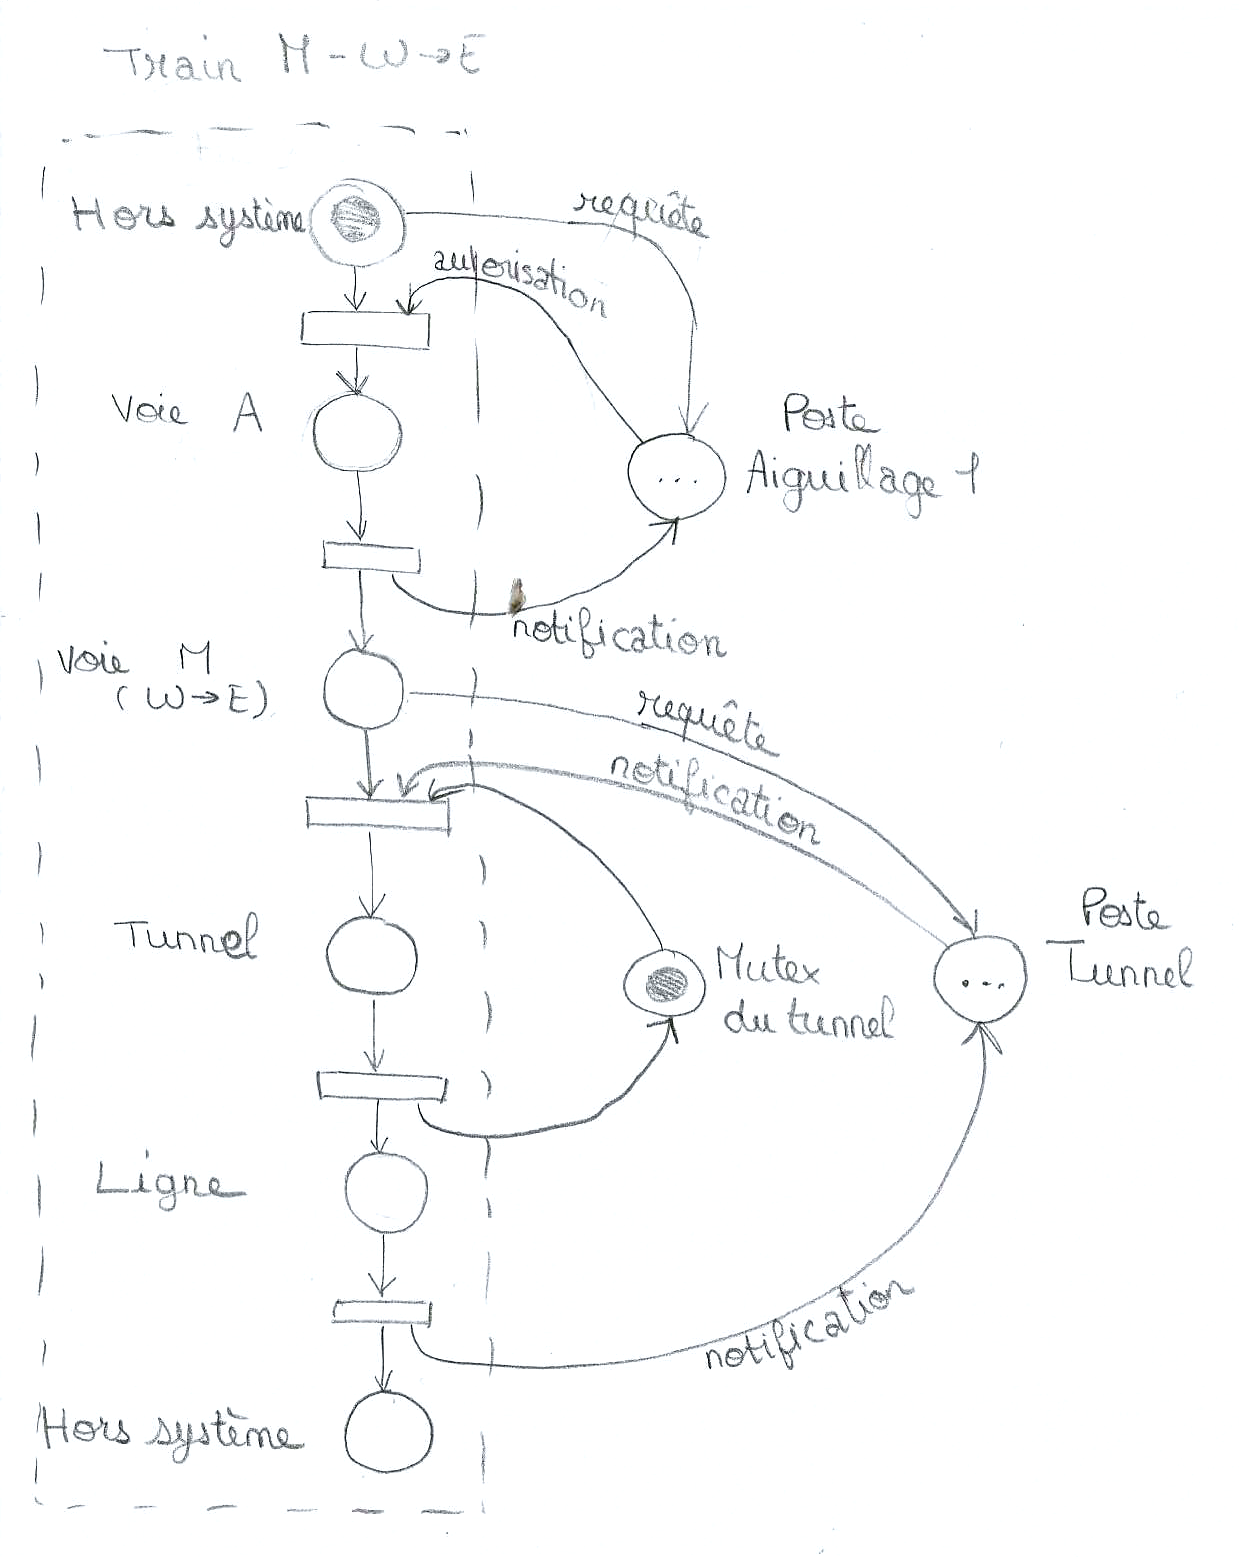
\includegraphics[width=.5\linewidth]{img/reseau_petri.png}
	\caption{Réseau de Petri appliqué au cas des trains de marchandise sur le W $\rightarrow$ E}
\end{figure}

\section{Le processus train}

\subsection{Initialisation, interruption et terminaison}

Le processus train prend en argument le nom du fichier de trains à lire. Il va ensuite mettre en place un handler pour SIGINT qui attendre les threads et permettra de libérer toutes les ressources qui alloue avant de se terminer en cas d'interruption. Ensuite, il initialise un Parser qui permet de lire, train par train, les caractéritiques des trains qui doivent être envoyées dans le système. Afin de conserver les identifiants des threads de trains qui vont être lancées, un tableau est alloué à la taille indiquée par le Parser. Ensuite, chaque train est lancée au moment indiqué dans le fichier (voire paragraphe suivant). Si une erreur de lecture se produit, le train qui était alors en train d'être lancé est abandonné et le programme passe directement au train suivant.

Le fichier se compose de la manière suivante :

\begin{itemize}
	\item 1er ligne : <nombre de trains n>
	\item n lignes suivantes : <moment du lancement> <type de train> <sens de circulation>
\end{itemize}

Le moment du lancement du train correpond à un nombre de secondes après le début du programme. Les trains doivent être classés dans leur ordre de lancement (moments de lancements croissants).

Lorsque tous les trains sont lancées, la thread principale du processus train se met en attente de toutes ses threads de trains ou d'un signal d'interruption SIGINT. Si un signal SIGINT est reçu, un signal SIGTERM est envoyé à toutes les threads de trains.

\subsection{Les threads du processus train}

Chaque thread de train a un comportement prédéfini en fonction de son type (Marchandise, Grande Ligne ou TGV). Cependant, on trouve des comportements communs entre tous les trains :
\begin{itemize}
	\item Tous les trains sont considérés comme en dehors du sytème à leur démarrage. Il doivent recevoir une autorisation de la zone critique la plus proche pour entrer dans le système.
	\item Lorsqu'un train arrive aux abord d'une zone critique, il s'arrête et envoie une requête à la zone critique en question au travers de la file de message inter-processus.
	\item Après avoir quitté une zone critique, le train envoie une notification au manager de la zone critique.
	\item Les trains doivent recevoir une autorisation et aquérir un mutex pour passer le tunnel afin qu'il n'y ait qu'un seul train à la fois dans le tunnel.
\end{itemize}
Une thread de train se termine d'elle même lorsque le train quitte le système.

\section{Le processus manager}

\subsection{Initialisation, interruption et terminaison}

Le processus manager ne prend pas d'arguments. Durant l'initialisation, il initialise les cinq compteurs des zones critiques, le mutex de protection de ces compteurs. Ensuite, un handler de SIGINT est mis en place de manière à ce que, si un signal SIGINT survient, les trois threads de manager sont terminées et le processus manager se termine. Enfin, les trois threads de manager sont créées et lancées dans leur méthode.

Lorsque tous les trains auront fini de passer, le processus manager va recevoir un SIGINT qui sera alors attrapé (cf. ci-dessus) et les différentes threads seront terminées proprement.

\subsection{Les threads du processus manager}

Les trois threads du manager (aiguillage 1, aiguillage 2 et tunnel) ont une unique fonction en commun. En arrivant sur cette fonction, les trois threads vont << se connecter >> à la file de message et effectuer indéfiniement (jusqu'à recevoir un signal de fin) les instructions suivantes :

\begin{enumerate}
    \item récupérer le contenu de la file de message qui est destiné au manager ;
    \item traiter toutes les notifications dans l'ordre où elles arrivent et stocker les requêtes dans une liste de messages ;
    \item traiter toutes les requêtes de la liste de messages dans l'ordre de priorité (TGV puis GL puis M).
\end{enumerate}

Ainsi, à la fin de chaque itération pour une thread donnée, cette thread a traitée tous les messages qui lui étaient destinés au début de l'itération.

\subsubsection{Réception et résolution des messages}

La réception des messages se fait, comme expliqué plus haut, par le stockage dans une liste de messages (structure créée pour l'occasion). Les messages de notification sont alors tous traités de manière à libérer le plus de zones critiques possibles.

Ensuite, les requêtes précédemment stockées dans la liste de message sont lues une par une et les requêtes sont traitées par priorité décroissante. Si une requête ne peut donner lieu à une autorisation de passer, elle est remise dans la liste de message pour être traitée ultérieurement.

\section{Améliorations possibles}

Actuellement, les processus ne bloquent jamais les signaux. Il pourrait être intéressant d'ignorer les SIGINT par exemple pendant les phases d'initialisation et de terminaison des processus pour assurer une meilleure sécurité.

Beaucoup de variables sont stockées en publique, ce qui peut être problématique car tous les processus y ont un accès. On pourrait penser à des passages par arguments pour réduire le nombre de variable globales.
\end{document}
